\documentclass[english]{article}\usepackage[]{graphicx}\usepackage[]{color}
\usepackage{alltt}
\usepackage[T1]{fontenc}
\usepackage[latin9]{inputenc}
\usepackage{geometry}
\geometry{verbose}
\setcounter{secnumdepth}{2}
\setcounter{tocdepth}{2}
\usepackage{amsmath}
\usepackage{graphicx}
\usepackage{esint}
\usepackage{algpseudocode}
\usepackage{algorithm}
\usepackage{babel}
\usepackage{verbatim} % for \begin{comment}
\usepackage{subcaption}
\usepackage{float}
\IfFileExists{upquote.sty}{\usepackage{upquote}}{}
\begin{document}

\title{Autonomous Robots and Environmental Mapping}

\author{M. Horning, M. Lin, S. Srinivasan, S. Zou}

\maketitle

\begin{abstract}

Compressed sensing is a technique used to reconstruct sparse signals and images while sampling well below the Nyquist rate. Commonly used in fMRIs and medical imaging, we aim to use this technique to allow autonomous robots to map piecewise constant areas of interest within a larger environment. In our experiment, we programmed a robot equipped with a reflectance sensor to travel along straight-line paths on a black testbed with white regions of interest. The robot integrated sensor readings and sent that sum to a remote server after each path. Each data point consists of the robot's start and end positions, tracked by an overhead camera, and the integral found along that path. Once all the data has been collected, the environment is reconstructed by minimizing the sum of the data fitting term and an L1 penalty term. We also implemented an "adaptive path selection scheme", allowing the robot to more intelligently target regions of interest based on the data collected from an initial set of random paths. Preliminary simulations of our experiment show reconstruction of 100x100 images with only 100 data points (relative err. = 0.28), and we have begun trials with data collected by the robot.

\end{abstract}

\pagebreak
\tableofcontents
\pagebreak

\section{Introduction}

\begin{comment}
Discuss Compressed Sensing
\end{comment}

Environment mapping is amongst the foundational problems of mobile robotics. In order for an autonomous vehicle to operate effectively within an environment, 

The task of mapping an unknown environment is well-studied in the area of autonomous robotics. 

Compressed sensing describes a technique in which a signal is reconstructed by solving an underdetermined linear system. Doing so allows a signal to be found from a relatively small amount of data. 

%%%%%%%%%%%%%%%%%%%%%%%%%%%%%%%%%%%% LAB SETUP %%%%%%%%%%%%%%%%%%%%%%%%%%%%%%%%%%%%%%%%%%%%%%%%%%%
\section{Lab Setup}
\subsection{Overview}
The setup in the UCLA Applied Mathematics Laboratory (AML) consists of three main components: 

\begin{itemize}
\item A robot vehicle on a black 1.5 m x 2.0 m rectangular test bed made of black asphalt felt paper
\item 2 Overhead Imaging Source DMK 21F04 1/4 Monochrome CCD cameras
\item A Server hosted on a Windows Computer
\end{itemize}

\subsection{Robot}

The robot itself consists of 5 main components:
\begin{enumerate}
\item \textbf{An Arduino Uno with an AdaFruit WiFi Shield:}
		The WiFi Shield allows the Arduino to connect to a network, and so communicate with the server. The WiFi Shield uses up digital pins 3, 4, 5, 10, 11, 12 and 13. Digital Pins 6, 7, 8, 9 connect to the Motor Controller, while analog pin 4 is used to connect to the reflectance sensor. The Arduino is powered by a 9V battery and has limited on-board processing power (16 MHz) and memory (32 KB Flash and 2 KB SRAM). The Arduino is uploaded with the code in \texttt{compressedSensing.ino} (see Appendix).
\item \textbf{Analog Reflectance Sensor:} The reflectance sensor measures the reflectance of the surface, but note that brighter (e.g. white) surfaces register low values while darker (e.g. black)  surfaces register higher values. To make the data more intuitive to understand, the data read is subtracted from the maximum reading (found experimentally) of the sensor, so that black surfaces get stored as lower values while white surfaces are stored as higher values. Currently, the raw data from the sensor is not used but instead thresholded so that any sensor readings above the threshold are read as white and those below are read as black. To extend the project to allow reconstruction of images with varying shades of grey, more thresholds will have to be created so that sensor readings within some range map to some colour between black and white.
\item \textbf{Chassis:} The chassis has four motors, that are powered by 5 AA 1.5V batteries. The chassis also has a switch to connect or disconnect the batteries from the motor.
\item \textbf{Motor controller:} The motor controller acts as the intermediary between the Arduino and motors. The board logic operates at 5V, provided by the Arduino but the AA batteries connect to the motor controller and are actually used to drive the motor. The two motors on the left and the two motors on the right are connected parallel to each other, so the voltage applied to a motor on the front will be the same as the voltage applied to a motor at the back on the same side. This setup provides tank steering for the robot. The motor controller has 4 inputs and 4 outputs. Each input maps to an output that controls the voltage applied to one terminal of the motor. As an example, the robot can be made to move forward by applying a high voltage on both the pins that connect to the positive terminal and a low voltage to both the pins that connect to the negative terminal. It can be made to rotate left by applying high voltage to the positive terminal and low voltage to the negative terminal on the left motors, and applying high voltage to the negative terminal and high voltage to the positive terminal. Note that this in contrast to other types of motor controllers that have two inputs for voltage and two inputs for direction to spin the wheels on either side.

\item \textbf{Tag (Visual ID):} A white rectangular tag with a black-tape border and a black header strip is mounted on the motor controller. It serves as a means for the overhead camera to visually identify the robot. Its distinctive shape and design make it hard to confuse with other shapes that appear on the test bed, and hence serves as unique way to identify the robot's position. Ideally, the center of the tag should be directly over the reflectance sensor -- the video camera should really be tracking the reflectance sensor's as it traverses the test bed collecting data.
\end{enumerate}

\subsection{Video Camera}
The cameras have a resolution of 640x480 pixels and a frame rate of 30 fps and are connected to a PC via
firewire. The computer runs \texttt{vehicle\_tracker.py}, a python script used to track the robots as
they move about the test bed. The script utilizes OpenCV to search for contours and recognize the tag
that is fixed on top of the vehicle, and return the robot's current position and orientation. The
orientation is found from the direction of the vector pointing from the tag's center to the header
strip's center. The script obtains three pieces of information by processing the video: the x-coordinate,
the y-coordinate and the heading and writes this data to a COM port in the form $*\$|x|y|\theta|!\textbackslash$n. The COM port should have a USB-Serial Cable plugged in that is connected to a Wi232 transceiver that transmits this serial data over radio.

\subsection{Server}

The server acts as the intermediary between the robot and video camera. The main script on the server is \texttt{robotServer.cgi}. The Arduino, upon connecting to the network will send a request to this script on the
server with its ``state'' and optionally ``data.'' Note that we do not need an internet connection for this project. Rather, it keeps things simpler if the robot and server are connected to the same priavte network. It is possible to host the server on a network with Internet connection, such as UCLA-MATHNET, but the robot ultimately also needs to be on the same network. If the robot and server need to be on different networks, port forwarding needs to be configured on the network that the server is on so that the Arduino's requests actually get sent to the server. This can be a hassle, so it is advised that the robot and server are on the same private network.

To obtain the robot's location, the server reads data from the serial port. The serial port should be connected to a Wi232 transceiver that receives data broadcast by the other Wi232 transceiver.

\subsection{Putting it all together}

We wish to collect some $m$ data points, where $m << n$, the dimension of the image. Each data point consists of the starting location of the robot, the final location of the robot and the sum of the reflectance sensor values obtained as it travelled in a straight line between the two points. The robot operates as a finite state machine. It consists of binary states, and they function as follows:
\begin{itemize}
\item State 0: When the robot is in state 0, it is either moving/turning to its new start position or requesting the server to confirm it position as it is about to start travelling along a new path and collect data. Note that when the robot is getting into its new start position, there is no communication with the server. This happens everytime the robot switches to state 0 from state 1.
\item State 1: When the robot is in state 1, it is either moving along a path collecting data or requesting the server that its position at the end of a path. Note that when the robot is travelling along a path collecting data, there is no communication with the server. This happens everytime the robot switches to state 1 from state 0.
\end{itemize}
The following flowchart shows the decision-making process of the robot:
\begin{figure}[H]
\begin{centering}

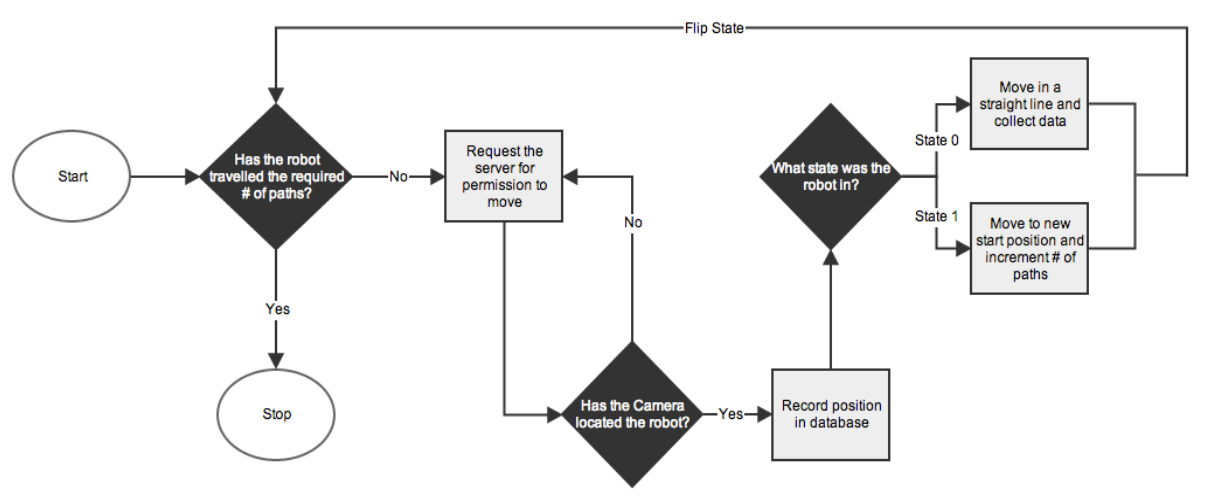
\includegraphics[width=1\linewidth]{figures/robot_flowchart}
\end{centering}

\caption{Flowchart of Robot's Logic}
\label{fig:robot-flowchart}
\end{figure}


\begin{comment}
Description of testbed, hardware, software, logic
Sid's flowchart
\end{comment}

\subsection{Noise}

Some of the factors that may affect the quality of the data collected are detailed below:
\begin{itemize}
\item \textbf{The test bed is not composed of perfectly black and white regions.} As a result, when the robot roams over what might appear to be a black region, the sensor might register a value less than the threshold and hence count it as black, or vice-versa. However, this should not cause any major issues as roaming over some distance over a white region yields sensor integral around two orders of magnitude above sensor integrals obtained by roaming over the same distance over a black region.
\item \textbf{Robot slows down with time.} The batteries wear out as the experiment goes on. So although we do not expect there to be a siginifcant difference in the speed between sucessive data points, when we consider the velocity of the robot at the first data point and its velocity at the 200th data point,there might be some difference in its velocity. The difference in velocity might be an issue as in our implementation, we integrate sensor readings over time, not distance. This would be appropriate if the velocity is constant which is a reasonable assumption for a low number of paths. But as the number of paths increases and velocity decreases, the robot would integrate fewer readings even though it travels for the same time. This will skew the data, but the seriousness of the issue has not been fully studied.
\item \textbf{Tag is not exactly centered over the sensor.} This is only a minor issue and can only be minimised to the extent that it not significant. This will not cause a constant systematic error as when the robot is travelling paths in different angles, the offset between the tag and sensor will vary. However, it is something to keep in mind and every attempt should be made to align the center of the tag with the sensor.
\end{itemize}



%%%%%%%%%%%%%%%%%%%%%%%%%%%%%%%%%%%%%%%%%%%%%%%%%%%%%%%%%%%%%%%%%%%%%%%%%%%%%%%%%%%%%%%%%%%%%%%%%%

\section{Models and assumptions}

\subsection{Problem Constraints}

Our model and lab setup were designed with the following constraints in mind: 
limited on board processing power, limited on board storage, and limited bandwidth 
(or infrequent communication with the main server). Real world examples where these constraints 
might exist include robot submarines that can only transmit data when they surface but given the massive amount of sensor information that would be collected whilst traveling in the ocean it becomes infeasible to store it all.  robot need only to sum up the the sensor readings it gets

\subsection{Mathematical Model}
Without loss of generality, we assume the area to be explored is a
rectangle denoted by $\Omega$, and the interested environment variable
$u(x,y)$ is a piece-wise constant function defined on $\Omega$.
See Figure \ref{fig:An-illustration-of-paths} for an illustration.
Assume the robot travels through $n$ different paths, which are denoted
by $C_{1},\ldots,C_{n}$. Along each path $C_{k}$, the integral of
environment variable $u$ is obtained, which is denoted by $b_{k}$.
The path integrals are written as
\begin{equation}
b_{k}=\int_{C_{k}}u(x,y)\mathrm{\,{d}\Gamma},\; k=1,\ldots,n.\label{eq:path-integral}
\end{equation}


\begin{figure}[h]
\begin{centering}

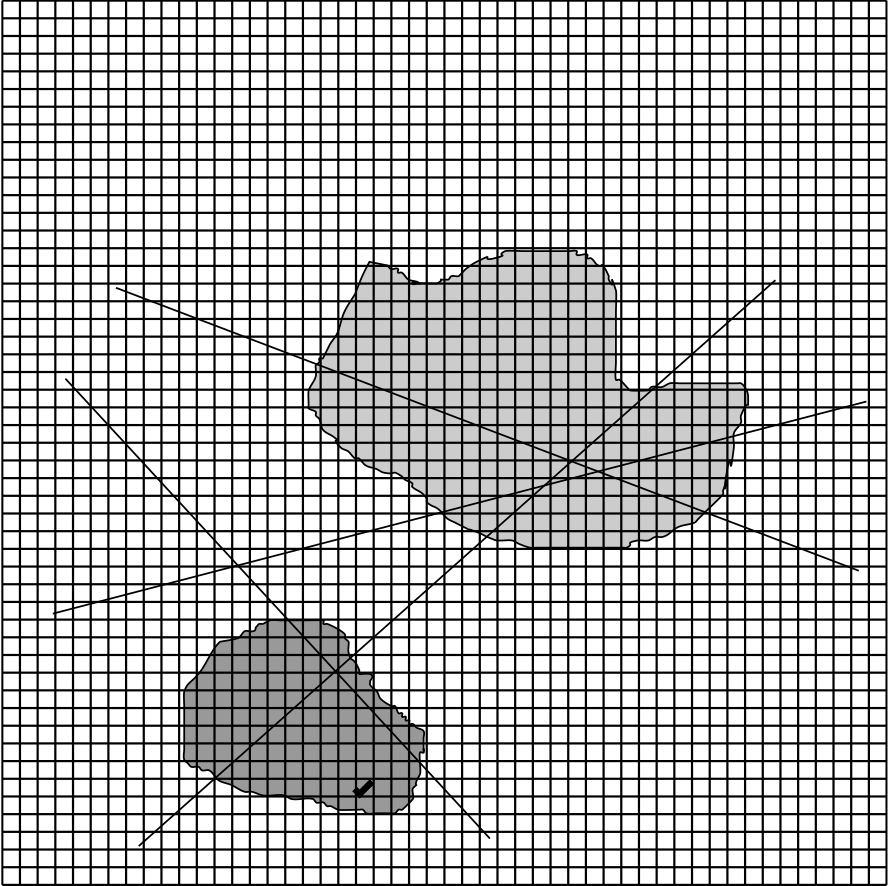
\includegraphics[width=0.5\linewidth]{figures/path-illustration}
\par\end{centering}

\caption{\label{fig:An-illustration-of-paths}An illustration of the paths
of robots. The shaded regions denote the area of interest (unknown),
where the values of environment variable $u$ is significantly different
from the surroundings. The size of the unit pixel (each small rectangle)
is determined by the accuracy of the positioning system.}
\end{figure}


For computational purpose, the whole domain is discretized into rectangular
pixels (See Figure \ref{fig:An-illustration-of-paths}). Each path
$C_{k}$ defines a weight $a_{k,ij}$ for each pixel $(i,j)$. If
$C_{k}$ does not intersect with pixel $(i,j)$, then $a_{k,ij}=0$,
otherwise $a_{k,ij}$ is defined to be proportional to the length
of the part of $C_{k}$ that falls within pixel $(i,j)$. It is also
assumed that the value of $u$ is a constant within each pixel $(i,j)$,
which is denoted by $u_{ij}$. After discretization, Eq (\ref{eq:path-integral})
becomes

\begin{equation}
b_{k}=\sum_{i}\sum_{j}a_{k,ij}u_{ij}.\label{eq:path-integral-discrete}
\end{equation}
Let $b=(b_{1},\ldots,b_{n})^{t}$, $u=(u_{ij})$, then $b$ and $u$
have a linear relation, which is written as 
\begin{equation}
Au=b,\label{eq:system-eq}
\end{equation}
where the linear operator $A$ is specified in Eq (\ref{eq:path-integral-discrete}).
Eq (\ref{eq:system-eq}) is the model equation, which poses an inverse
problem. In this equation, $b$ can be obtained from the experiment,
$A$ is determined by user-specified paths for the robot, which can
be calculated offline. $u$ is the variable that we want to solve.
Of course, if the paths form a complete raster scan over the whole
domain, then theoretically Eq (\ref{eq:system-eq}) has a unique solution.
For economical reasons, it is desirable to use much fewer paths and
still being able to reconstruct a solution for $u$. The problem is well suited for compressed sensing based image reconstruction techniques, which provide a way to solve these underdetermined systems, 

\begin{comment}
Description of constraints for our problem
limited bandwidth, data storage
Also assumptions about simple piecewise environments
\end{comment}

\section{Algorithm for solving the inverse problem}

Based on the observation that the image $u$ to be reconstructed is
piecewise constant, its directional gradients, $\nabla_x u$ and $\nabla_y u$, are sparse over
the domain. We also say that there is a second operator $\Psi$, where $\Psi u$
is also sparse. For simplicity, we assume that $\Psi = I$, due to the nature 
of our experiments with the autonomous robot. That is, we can easily 
enforce the sparsity of $u$ by adjusting the size of the areas of interest with 
relation to the size of the test bed. Inspired by the compressed sensing theory, we postulate
that the actual solution $u$ should minimize the energy functional 
\[E(u) = \alpha |u|_0 + \beta\left(|\nabla_x u|_0+|\nabla_y u|_0\right),\]
where $\alpha$ and $\beta$ are parameters specifically chosen based on the nature
of $u$.

Now, let $A$ be our measurement operator as described in the previous section, and let 
$b$ be the collected samples. Then, in order to reconstruct $u$, given that we have $A, b$, we must solve the optimization problem
\[ \underset{u}{{\text{{min }}}} E(u)\quad\text{such that}\; Au=b.\]
Solving this problem is intractible due to our use of the $\ell^0$ pseudo-norm, but we 
can relax it to an easily solved optimization problem by using a different sparsity-inducing 
objective function. We choose to use the $\ell^1$ norm or the nonconvex penalty function
$\varphi_p$ with $p \leq 1$, as described in the introduction. In order to account for noise 
in our data, we relax the constraint and instead use a penalty function to enforce data 
fidelity. Therefore, we can recover $u$ by solving the unconstrained optimization problem 
\begin{equation}
\underset{u}{{\text{{min }}}}\alpha\varphi_p\left(u\right)+\beta\varphi_p\left(\nabla_x u + \nabla_y\right)+\frac{\mu}{2}||Au-b||_2^2.\label{eq:minprob}\end{equation}
Although this is a nonconvex optimization problem in the case that $p<1$,
Chartrand \cite{chartrand2009fast} has shown that it can easily be solved, 
and that the solution will converge to the global minimum of the 
associated $\ell^0$ formulation. Therefore, we use the Split-Bregman method to reconstruct $u$. 

In order to use Split-Bregman, we rewrite \ref{eq:minprob} as
\begin{equation}
\underset{u,d,d_{x},d_{y}}{{\text{{min }}}}\alpha\varphi_p\left(d\right)+\beta\varphi_p\left(d_x + d_y\right)+\frac{\mu}{2}||Au-b||_2^2\quad\text{such that}\; d=u,\, d_{x}=\nabla_{x}u,\, d_{y}=\nabla_{y}u.
\label{eq:sbprob}\end{equation}
Then, we relax the constraints to
\[
\underset{u,d,d_{x},d_{y}}{{\text{{min }}}}\alpha\varphi_p\left(d\right)+\beta\varphi_p\left(d_x +
 d_y\right)+\frac{\mu}{2}\|Au-b\|_2^2 + \frac{\lambda_1}{2}\|d-u+b\|_{2}^{2}+\frac{\lambda_2}{2}\left(\|d_{x}-\nabla_{x}u+b_{x}\|_{2}^{2}+\|d_{y}-\nabla_{y}u+b_{y}\|_{2}^{2}\right),
\]
and then use our algorithm to reconstruct for $u$ through the following process:

\begin{algorithm}
\caption{Split-Bregman method}\label{split-bregman}
\begin{algorithmic}[1]
\Procedure{Split Bregman Solve}{$A,b$}\Comment{Solve \ref{eq:sbprob}}
\While{$\|u^k-u^{k-1}\|_2^2 < tol$}
\For{$n=1$ to $N$}
\State $u^{k+1}\gets \min_u{\frac{\mu}{2}\|Au-b\|_2^2+\frac{\lambda_1}{2}\|d-u+b\|_{2}^{2}+\frac{\lambda_2}{2}\left(\|d_{x}-\nabla_{x}u+b_{x}\|_{2}^{2}+\|d_{y}-\nabla_{y}u+b_{y}\|_{2}^{2}\right)}$
\State $d^{k+1}\gets \min_d{\alpha\varphi(d)+\frac{\lambda_1}{2}\|d-u+b\|_2^2}$
\State $d_x^{k+1}\gets \min_{d_x}{\beta\varphi(d_x)+\frac{\lambda_2}{2}\|d_x-\ \nabla_xu+b\|_2^2}$
\State $d_y^{k+1}\gets \min_{d_y}{\beta\varphi(d_y)+\frac{\lambda_2}{2}\|d_y-\ \nabla_yu+b\|_2^2}$
\EndFor
\State $b^{k+1}\gets b^{k}+\left(-d^{k+1}\right)$
\State $b_x^{k+1}\gets b_x^{k}+\left(\nabla_x \left(u^{k+1}\right) - d_x^{k+1}\right)$
\State $b_y^{k+1}\gets b_y^{k}+\left(\nabla_y \left(u^{k+1}\right) - d_y^{k+1}\right)$
\EndWhile
\EndProcedure
\end{algorithmic}
\end{algorithm}


And its associated Augmented Lagrangian functional $L(u,\, d,\, d_{x},\, d_{y},\, b,\, b_{x},\, b_{y})$ is 
\[\frac{\mu}{2}\|Au-g\|_{2}^{2}+\alpha|d|_{1}+\beta(|d_{x}|_{1}+|d_{y}|_{1})+\frac{1}{2}\lambda_{1}\|d-u+b\|_{2}^{2}+\frac{{1}}{2}\lambda_{2}(\|d_{x}-\nabla_{x}u+b_{x}\|_{2}^{2}+\|d_{y}-\nabla_{y}u+b_{y}\|_{2}^{2}).
\]
The solution process is iterative, with each iteration consisting
of three major steps:


\section{Results}
\subsection{Simulated Results}

\begin{figure}[h]
\centering
\begin{subfigure}{.22\textwidth}
  \centering
    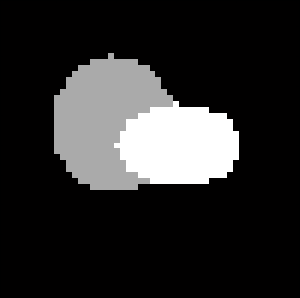
\includegraphics[width=1\linewidth]{figures/simulatedresultoriginal}
  \caption{50x50 test image.}
  \vspace{20pt}
  \label{fig:simulresorig}
\end{subfigure}%
\hspace{10pt}
\begin{subfigure}{.22\textwidth}
  \centering
    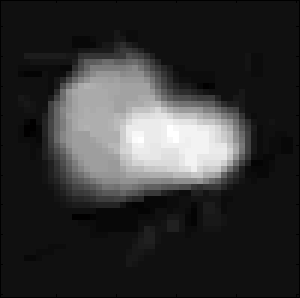
\includegraphics[width=1\linewidth]{figures/simulatedresultrec}
  \caption{Simulated reconstruction.}
  \vspace{10pt}
  \label{fig:simulresrec}
\end{subfigure}% 
\hspace{10pt}
\begin{subfigure}{.22\textwidth}
  \centering
    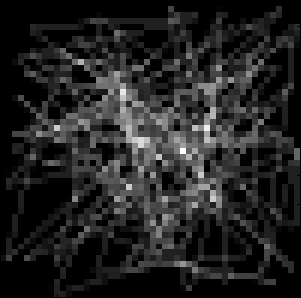
\includegraphics[width=1\linewidth]{figures/simulatedresultpaths}
  \caption{100 random paths used for simulated reconstruction.}
  \vspace{0pt}
  \label{fig:simulrespath}
\end{subfigure}%
\hspace {10pt}
\begin{subfigure}{.22\textwidth}
  \centering
    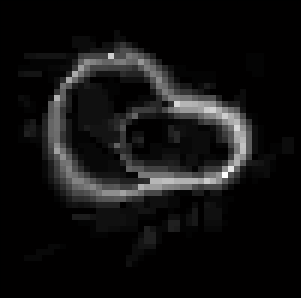
\includegraphics[width=1\linewidth]{figures/simulatedresulterror}
  \caption{Difference between the original image and the reconstruction.}
  \vspace{0pt}
  \label{fig:simulreserr}
\end{subfigure}
\caption{Simulated reconstruction using random paths.}
\label{fig:simulres}
\end{figure}

Before actually using the robot to collect data, we ran simulated reconstructions. Figure ~\ref{fig:simulresorig} is a 50x50 test image that we used for simulations. Although the lab setup required that the test bed consist of only black and white areas, in simulation, multiple shades of gray were used. Assuming the robot is capable of differentiating between the colors, the reconstruction will work just as well as it would with a black and white image.

Figure ~\ref{fig:simulresrec} is a reconstruction from 100 random paths. It is somewhat blurry, but it does reasonably well in determining the shape of the regions of interest as well as the colors of the regions. The image, being a 50x50 image, has 2500 pixels for which values must be determined. Thus, the image is being recovered from 100 data points, a 4:100 ratio of data points to values in the image.

We use Figure ~\ref{fig:simulrespath} to visualize the paths that were used in the reconstruction. For this reconstruction, the paths were generated by randomly selecting a starting point and then proceeding to randomly generate points to go to next. Thus, successive paths are connected with the end point of one path being the starting point of the next. In the figure, brighter pixels are pixels that are hit more frequently by the set of paths. Thus, this visual representation of the paths allows us to readily see what areas are more thoroughly examined and which are not.

Figure ~\ref{fig:simulreserr} shows the difference between the original image and the reconstruction. It makes it fairly clear that most of the error in the reconstruction is around the edges of the region of interest. As a means of quantifying the error, we found the norm of this difference and divided by the norm of the original image. In this particular case, this error value came to 0.2715.



\subsection{Experimental Results}

\begin{figure}[h]
\centering
\begin{subfigure}{.22\textwidth}
  \centering
    
\includegraphics[width=1\linewidth]{figures/experimentalresultoriginal}
  \caption{Image of the testbed, sized at 70x90.}
  \vspace{20pt}
  \label{fig:experresorig}
\end{subfigure}%
\hspace{10pt}
\begin{subfigure}{.22\textwidth}
  \centering
    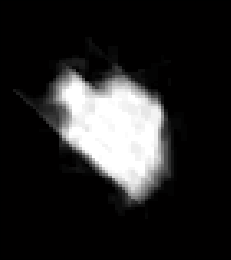
\includegraphics[width=1\linewidth]{figures/experimentalresultsimulation}
  \caption{Simulated reconstruction from the 178 paths that the robot travelled.}
  \vspace{0pt}
  \label{fig:experressim}
\end{subfigure}%
\hspace{10pt}
\begin{subfigure}{.22\textwidth}
  \centering
    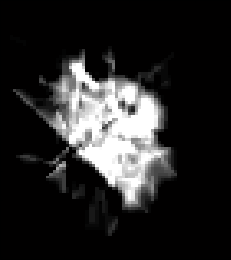
\includegraphics[width=1\linewidth]{figures/experimentalresultrec}
  \caption{Reconstruction from the data collected by the robot.}
  \vspace{10pt}
  \label{fig:experresrec}
\end{subfigure}%
\hspace {10pt}
\begin{subfigure}{.22\textwidth}
  \centering
    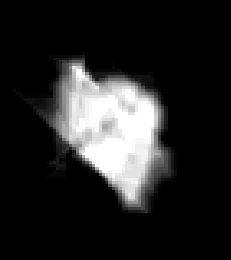
\includegraphics[width=1\linewidth]{figures/experimentalresulttunedrec}
  \caption{Reconstruction from the data collected by the robot using tuned parameters.}
  \vspace{0pt}
  \label{fig:experrestuned}
\end{subfigure}
\caption{Reconstruction using the data collected by the robot.}
\label{fig:experres}
\end{figure}

Having confirmed that our reconstruction algorithm works, we proceeded to carry out experimental testing with the actual robot. Figure ~\ref{fig:experresorig} shows a testbed that we used. The reconstruction for this testbed was carried out as a 70x90 image. As with previous simulations, the paths were generated randomly and such that the end point of one path was the starting point of the next path. This allowed the robot to gather data without having to reposition itself between paths.

As a means of comparison, we first carried out the reconstruction as a simulation, shown in Figure ~\ref{fig:experressim}. This simulated reconstruction uses the same set of 178 paths that the robot travelled along. Thus, this reconstruction is an ideal reconstruction. If the robot were able to pick up sensor values exactly as expected and with no noise, this would be the reconstruction found.

However, if we use the robot data alongside the same set of parameters as the simulated reconstruction, we instead find Figure ~\ref{fig:experresrec}. Clearly, this reconstruction is very noisy, giving black spots in the middle of the region and creating white spots where it should be black. This is due to the fact that the data collected by the robot is not as perfect as the data in simulation. As such, we retry the reconstruction, but with a lowered data fidelity parameter. This yields Figure ~\ref{fig:experrestuned}. Because there is less emphasis on fitting the image to the data, the reconstruction does a much better job. It is still not quite as accurate as the simulated reconstruction, but it is much cleaner than ~\ref{experresrec} and it still does a reasonably good job of showing the region of interest.


\section{Comparison with Other Approaches}
\begin{comment}
\end{comment}

In order to judge the effectiveness of our approach, we examine other methods of collecting data and reconstructing an image. Perhaps the most intuitive manner in which to gather data about the image is to sample individual points rather than travelling and integrating along a path. As when collecting data in the form of path integrals, we would want the number of sampled points to be as low as possible. Having sampled points for data, there are then multiple approaches to recovering the image. One approach is to simply use the same Split Bregman iteration that we are using for reconstruction from path integrals, but with the individually sampled pixels. Alternatively, we can take the value found at each pixel and assign the same value to nearby pixels, a method that we refer to as pixel expansion.

\begin{figure}
\centering
\begin{subfigure}{.45\textwidth}
  \centering
    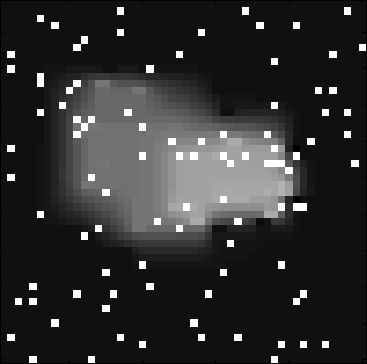
\includegraphics[width=1\linewidth]{figures/randompointreconstruction}
  \caption{Reconstruction using points sampled randomly.}
  \label{fig:randrec}
\end{subfigure}%
\hspace{10pt}
\begin{subfigure}{.45\textwidth}
  \centering
    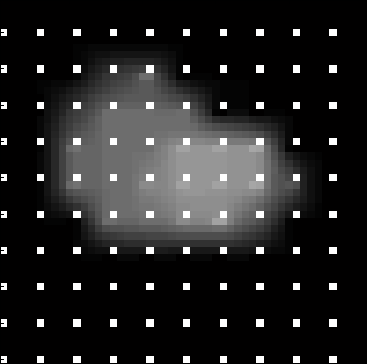
\includegraphics[width=1\linewidth]{figures/gridpointreconstruction}
  \caption{Reconstruction using points sampled on a grid.}
  \label{fig:gridrec}
\end{subfigure}
\caption{Values are found at sampled points, and Split Bregman iteration is used to reconstruct the image.}
\label{fig:samplerec}
\end{figure}

\begin{figure}
\centering
\begin{subfigure}{.45\textwidth}
  \centering
    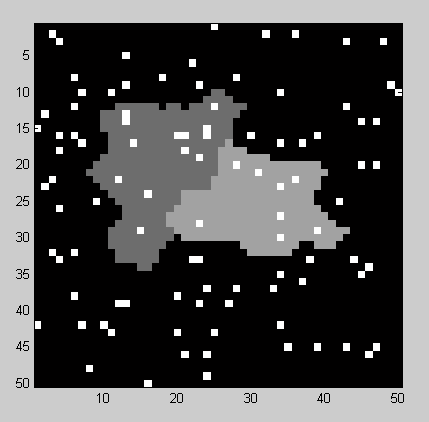
\includegraphics[width=1\linewidth]{figures/randompointexpansion}
  \caption{Expansion of points sampled randomly.}
  \label{fig:randexp}
\end{subfigure}%
\hspace{10pt}
\begin{subfigure}{.45\textwidth}
  \centering
    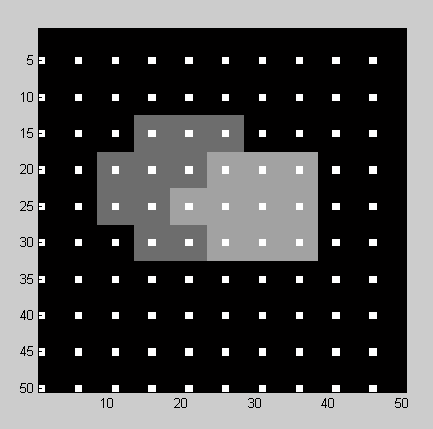
\includegraphics[width=1\linewidth]{figures/gridpointexpansion}
  \caption{Expansion of points sampled on a grid.}
  \label{fig:gridexp}
\end{subfigure}
\caption{Values are found at sampled points, and those values fill the area surrounding the sampled points.}
\label{fig:sampleexp}
\end{figure}

Figures \ref{fig:samplerec} and \ref{fig:sampleexp} present reconstructions of the previously shown 50x50 test image, Figure \ref{fig:simulresorig}, using these approaches, both with randomly sampled points and points sampled on a grid. In all cases, 100 pixels are sampled, and the sampled points are colored white.

In Figure \ref{fig:samplerec}, Split Bregman iteration was used with the collected data for reconstruction. The algorithm itself is unchanged, but the equation corresponding to a data point will simply give the value of a pixel rather than weighting pixels along the path. This method provides a moderately good reconstruction, especially in determining the general shape of the region of interest in the environment, but the demarcation between the shades of gray in the image is difficult to distinguish, making the image seem very blurry. This is not surprising because by sampling pixels, the only information gathered is about those specific pixels, so the space in between can gradate as quickly or slowly as the reconstruction algorithm deems fit. By comparing Figures \ref{fig:randrec} and \ref{fig:gridrec}, it seems that the reconstruction is more accurate when the points are sampled on a grid. This is reasonable because by sampling on a grid, the spread of sampled points is very even and well distributed. When the points are sampled randomly, certain areas will be less thoroughly investigated than others, hindering accurate reconstruction.

Figure \ref{fig:sampleexp} illustrates pixel expansion. This is done by looping through every pixel in the image, and for each pixel, finding and assigning the value from the nearest pixel that was sampled. This process creates expanded pixels of a single color around each sampled pixel. When the pixels are sampled on a grid, the even distribution causes the expanded pixels to simply be squares, essentially creating a low resolution version of the image, as in Figure \ref{fig:gridexp}. Figure \ref{fig:randexp} is a result of pixel expansion with randomly sampled pixels. The unpredictable spread of sampled pixels causes the expanded pixels to vary widely in shape and size, and the reconstruction does a poor job of determining the shape of the region of interest.

To compare these methods, Figure \ref{fig:othermethoderror} plots the error of these approaches, as well as the path integral reconstruction that we are actually carrying out, with respect to the number of data points collected. The blue line represents reconstruction from randomly generated path integrals, and as desired, for a low number of data points, it has lower error than the other methods. As the number of samples grows, all methods begin to have similar error; this is expected because any method will work reasonably well with enough data. Worth noting is that while pixel expansion from samples on a grid appears to do better than random path integrals for some of the low data situations, the effectiveness of grid point expansion is highly variable, and as such, its overall usefulness is limited. The accuracy of reconstruction is very dependent on how well the grid aligns with the given image, and choosing the best grid size for a given environment would require prior knowledge of the environment. Another flaw with pixel expansion is the dependence on accurate sampling; pixel expansion will be very heavily affected by noise. If a pixel is sampled inaccurately, the entire expanded pixel associated with that sample will be inaccurately reconstructed. Using Split Bregman iteration mitigates this issue, and using path integrals further diminishes the impact that a single inaccurate sample can have.


\section{Adaptive Pathing}
\begin{comment}
\end{comment}

\subsection{Simulated Results}
\begin{figure}
\centering
\begin{subfigure}{.22\textwidth}
  \centering
    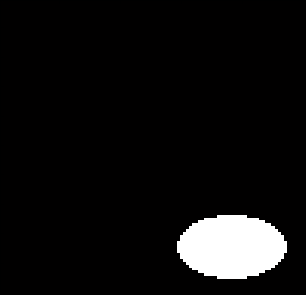
\includegraphics[width=1\linewidth]{figures/adaptiveresultoriginal}
  \caption{100 x 100 pixel test image with the area of interest in bottom right corner.}
  \vspace{0pt}
  \label{fig:adp_sim_orig}
\end{subfigure}%
\hspace{10pt}
\begin{subfigure}{.22\textwidth}
  \centering
    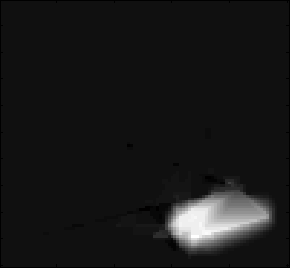
\includegraphics[width=1\linewidth]{figures/nonadaptiveresultrec}
  \caption{Simulated reconstruction from the 200 paths}
  \vspace{0pt}
  \label{fig:adp_randpaths_sim_rec}
\end{subfigure}%
\hspace{10pt}
\begin{subfigure}{.22\textwidth}
  \centering
    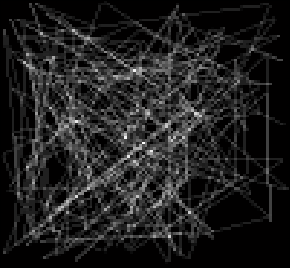
\includegraphics[width=1\linewidth]{figures/nonadaptiveresultpath}
  \caption{The 200 randomly generated paths.}
  \vspace{0pt}
  \label{fig:adp_randpaths_sim}
\end{subfigure}%
\hspace {10pt}
\begin{subfigure}{.22\textwidth}
  \centering
    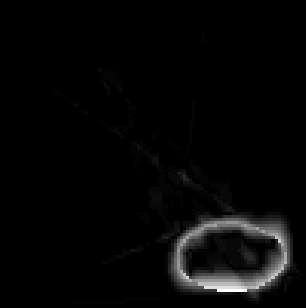
\includegraphics[width=1\linewidth]{figures/nonadaptiveresulterror}
  \caption{Difference between the original image and the reconstruction}
  \vspace{0pt}
  \label{fig:adp_randpaths_diff}
\end{subfigure}%
\caption{Simulated reconstruction using random paths as before.}
\label{fig:adp_randpaths_fig}
\begin{subfigure}{.22\textwidth}
  \centering
    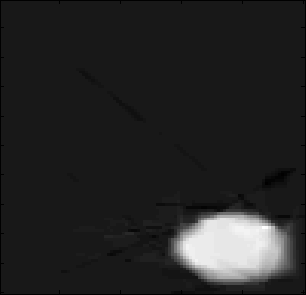
\includegraphics[width=1\linewidth]{figures/adaptiveresultrec}
  \caption{Simulated reconstruction from 200 adaptive paths.}
  \vspace{0pt}
  \label{fig:adp_adpaths_sim_rec}
\end{subfigure}%
\hspace{10pt}
\begin{subfigure}{.22\textwidth}
  \centering
    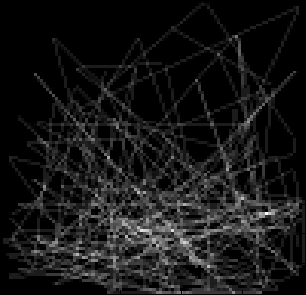
\includegraphics[width=1\linewidth]{figures/adaptiveresultpath}
  \caption{The 200 adaptive paths.}
  \vspace{0pt}
  \label{fig:adp_adpaths}
\end{subfigure}%
\hspace {10pt}
\begin{subfigure}{.22\textwidth}
  \centering
    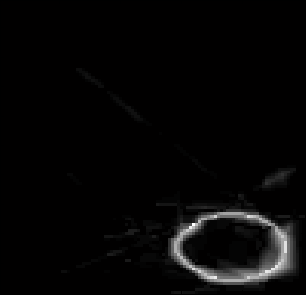
\includegraphics[width=1\linewidth]{figures/adaptiveresulterror}
  \caption{The difference between the reconstruction and original image.}
  \vspace{0pt}
  \label{fig:adp_adpaths_sim_diff}
\end{subfigure}
\caption{Reconstruction using the adaptive paths.}
\label{fig:adp_adpaths_sim_fig}

\end{figure}


\subsection{Experimental Results}

\begin{figure}
\centering
\begin{subfigure}{.4\textwidth}
  \centering
    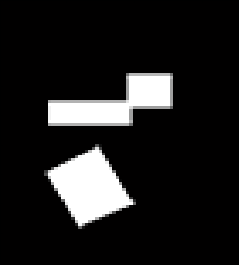
\includegraphics[width=1\linewidth]{figures/adaptiveexperimentalresultoriginal}
  \caption{Image of the testbed, sized at 70x90}
  \vspace{0pt}
  \label{adp_exp_orig}
\end{subfigure}%
\hspace{10pt}
\begin{subfigure}{.4\textwidth}
  \centering
    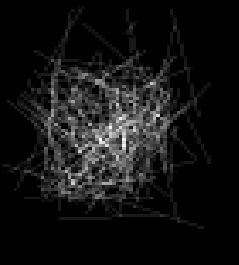
\includegraphics[width=1\linewidth]{figures/adaptiveexperimentalresultpath}
  \caption{The 224 adaptive paths traveled by the robot}
  \vspace{0pt}
  \label{adp_exp_paths}
\end{subfigure}%
\hspace{10pt}
\begin{subfigure}{.3\textwidth}
  \centering
    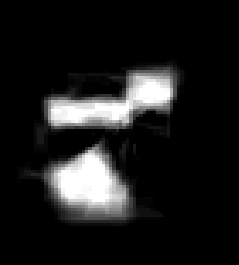
\includegraphics[width=1\linewidth]{figures/adaptiveexperimentalresultsimulation}
  \caption{Simulated reconstruction for the adaptive paths traveled by the robot}
  \vspace{0pt}
  \label{}
\end{subfigure}%
\hspace{10pt}
\begin{subfigure}{.3\textwidth}
  \centering
    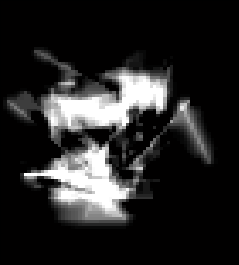
\includegraphics[width=1\linewidth]{figures/adaptiveexperimentalresultrec}
  \caption{Image reconstruction using robot collected data}
  \vspace{0pt}
  \label{adp_exp_recon_untuned}
\end{subfigure}%
\hspace {10pt}
\begin{subfigure}{.3\textwidth}
  \centering
    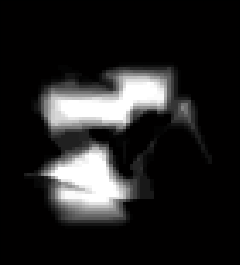
\includegraphics[width=1\linewidth]{figures/adaptiveexperimentalresulttunedrec}
  \caption{Image reconstruction using robot collected data with tuned parameters}
  \vspace{0pt}
  \label{adp_exp_recon_tuned}
\end{subfigure}
\caption{Experimental results of adaptive pathing using robot collected data}
\label{adp_exp_fig}
\end{figure}

\section{Conclusions and Further Work}

\newpage
\bibliographystyle{plain}
\bibliography{resources.bib}


\newpage
\textbf{Appendix}


\end{document}
